\section{Circle results}
\label{section:Circle_results}
\subsection{Drag and lift}
We start by looking at time-series plots of drag and lift of nonspinning and spinning circular cylinders as Fig. \ref{fig:timens} and \ref{fig:times} show. We observe when $Fr^2$ is in the range of $[0.7, 3]$, the flow is in an unsteady, transitional flow regime. At $Fr^2 = 10$, the drag takes a while to reach a quasi-steady state. Oscillations in drag and lift occur when $Fr^2 > 1$ due to vortex-shedding. The oscillation amplitudes are larger for lift than for drag because the release of the vorticies alternates between the top and bottom of the body. The larger lift amplitudes at $Fr^2 > 10$ are explained by the fact that more stratification suppresses vortex shedding. When we have little or no stratification, the vorticies are freer to travel vertically. As expected, there is no oscillation in lift at $Fr^2 < 0.7$. The introduction of spin at $Fr^2 > 1$ increases the amplitude of the oscillation in drag. The introduction of spin also causes the lift at $Fr^2 = 10$ to take longer to converge to a quasi-steady average value. Based on these plots, we conclude the vortex-shedding transition for a spinning circle occurs somewhere in the range $Fr^2 \in (3,7)$. 

We now compare the drag and lift means between spin and no spin across different $Fr^2$ as Fig. \ref{fig:circleforces} shows. We observe the addition of spin affects the average lift but not the average drag, and there is no lift when spin is absent. These two observations are consistent with the Kutta–Joukowski theorem. The effects of stratification particularly manifest themselves when $Fr^2 < 1$. The substantial increase in drag with increase in stratification due to \textit{upstream blocking}, or \textit{vertical confinement} is a well-known phenomenon \cite{deng_drag_2022, ortiz-tarin_stratified_2019}. These plots show that differences in the flow between $Fr^2 = 100$ and homogeneous flow are negligible. This suggests that flows at $Fr^2 = 100$ can be approximated as homogeneous. We look at the comparison of static and spinning pressure plots for circular bodies in Fig. \ref{fig:circle_pressure}. The pressure distributions change marginally as $Fr^2$ decreases until $Fr^2 = 0.1$. At this point, a transition occurs in the pressure distribution. The isobaric regions become flattened due to stratification limiting vertical fluid interaction by means of a potential energy barrier. This leads to a buildup of pressure in front of the body. This effect increases when $Fr^2 = 0.01$. 

As stratification increases, there is an overall negative trend in lift. The key difference between the spin and no spin cases is the presence of a strong negative pressure field above the spinning bodies. This negative pressure zone is the main phenomenon behind the lift seen in earlier plots and is a result of the Magnus effect. This relative low pressure zone goes away when $Fr^2 < 1$ as stratification increases. 
\begin{figure}
    \centerline{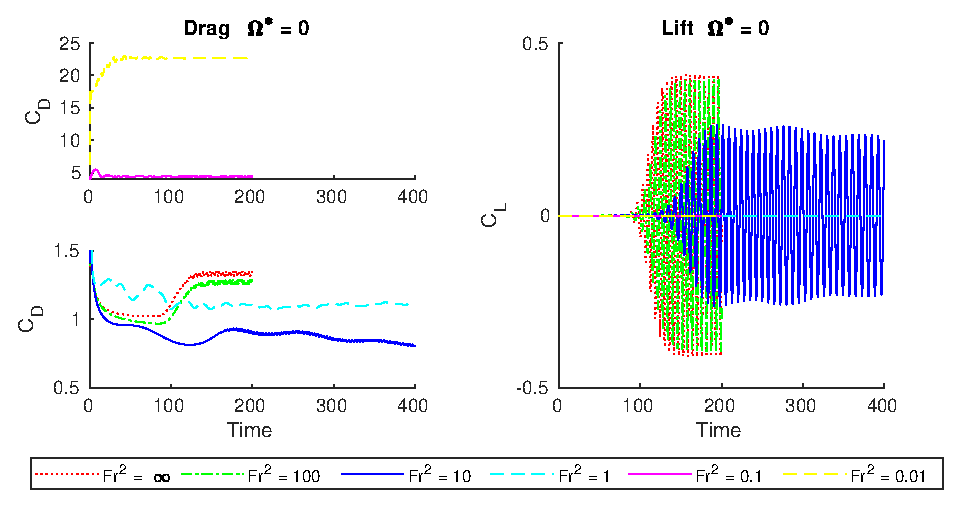
\includegraphics[width=\textwidth]{images/circle/timens.eps}}
    \caption{Time series data for nonspinning circle}
    \label{fig:timens}
\end{figure}
\begin{figure}
    \centerline{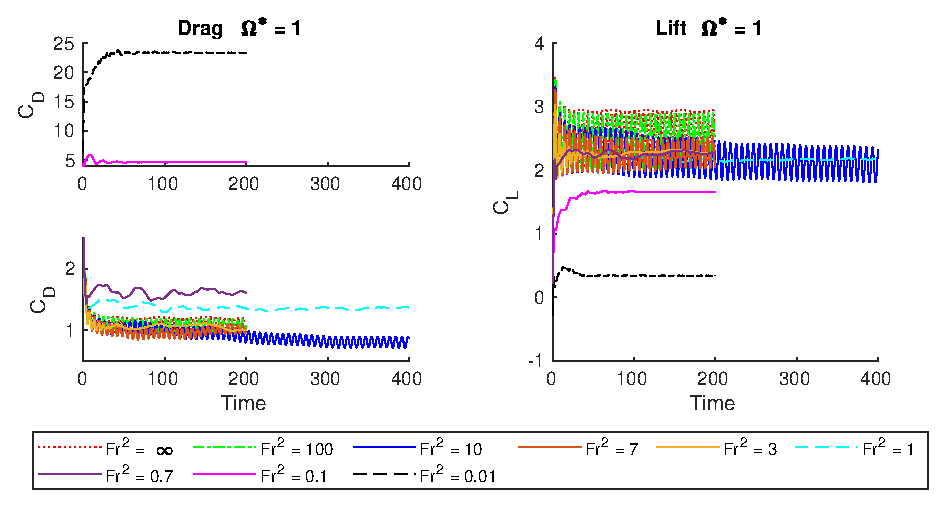
\includegraphics[width=\textwidth]{images/circle/times.eps}}
    \caption{Time series data for spinning circle}
    \label{fig:times}
\end{figure}

\begin{figure}
    \centering
    \begin{subfigure}[b]{0.49\textwidth}
        \centering
        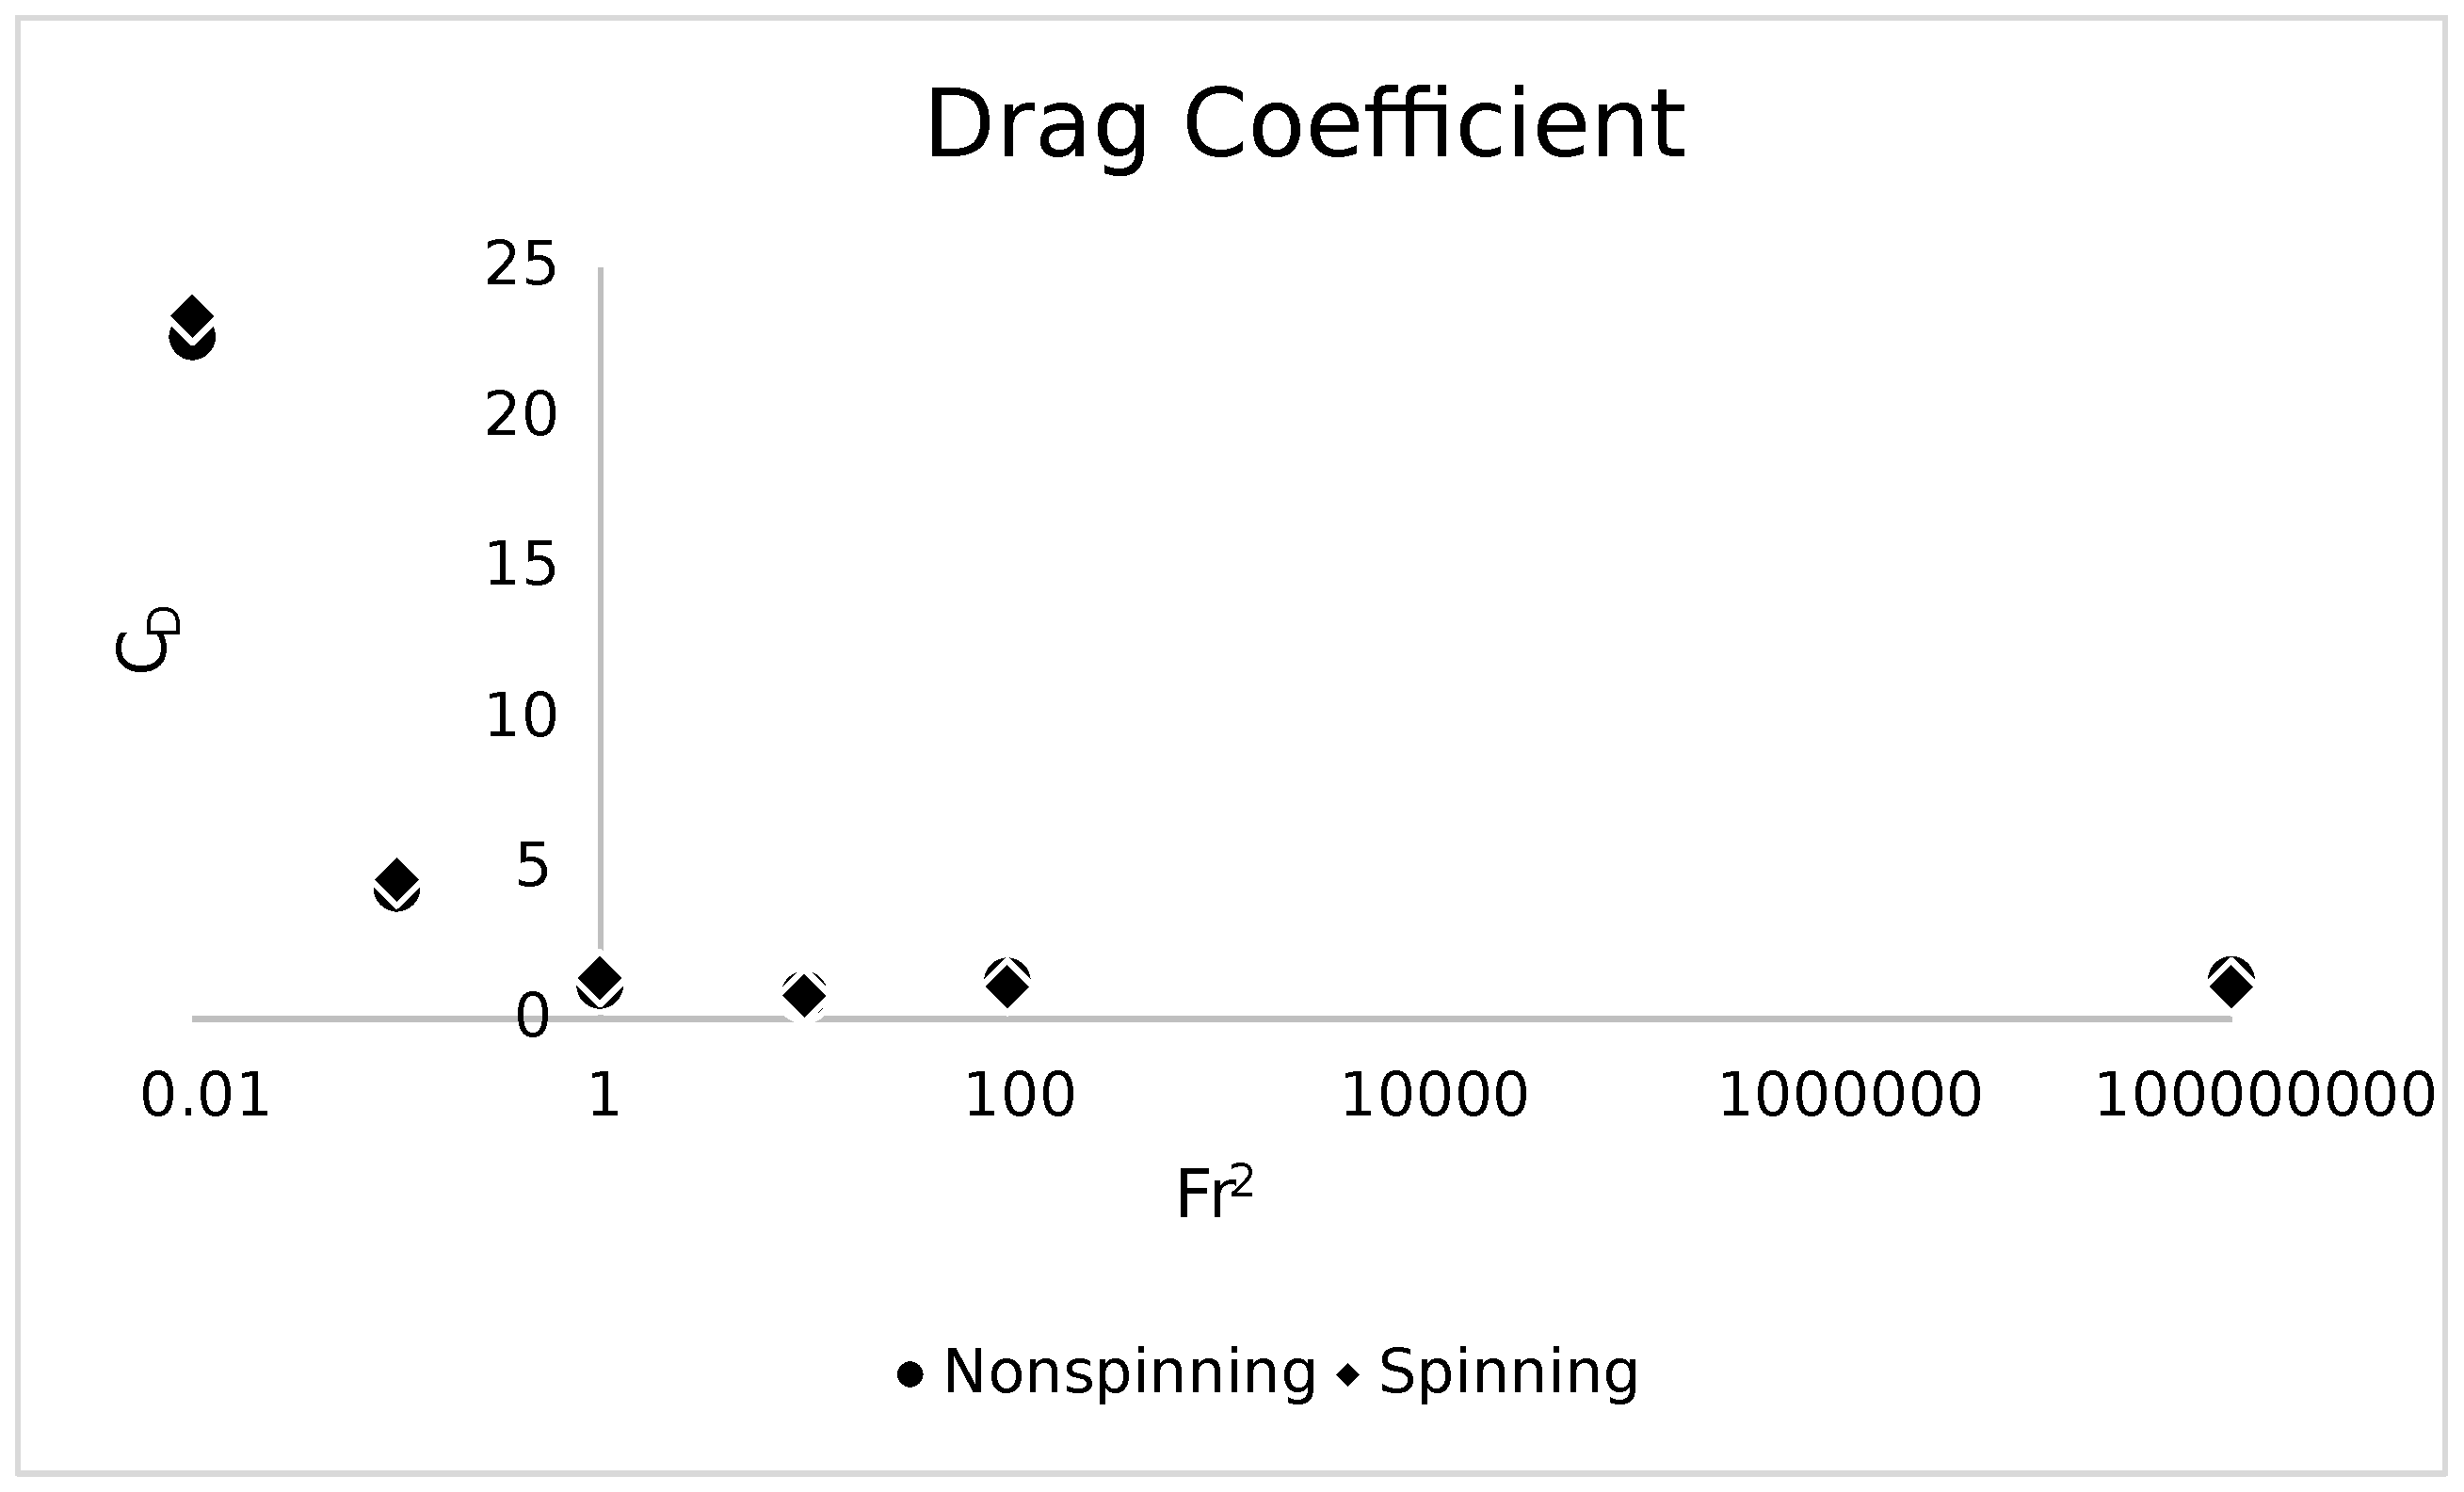
\includegraphics[width=\textwidth]{images/circle/ar1drag.eps}
        \caption{Drag coefficients}
        \label{fig:ar1drag}
    \end{subfigure}
    \hfill
    \begin{subfigure}[b]{0.49\textwidth}
        \centering
        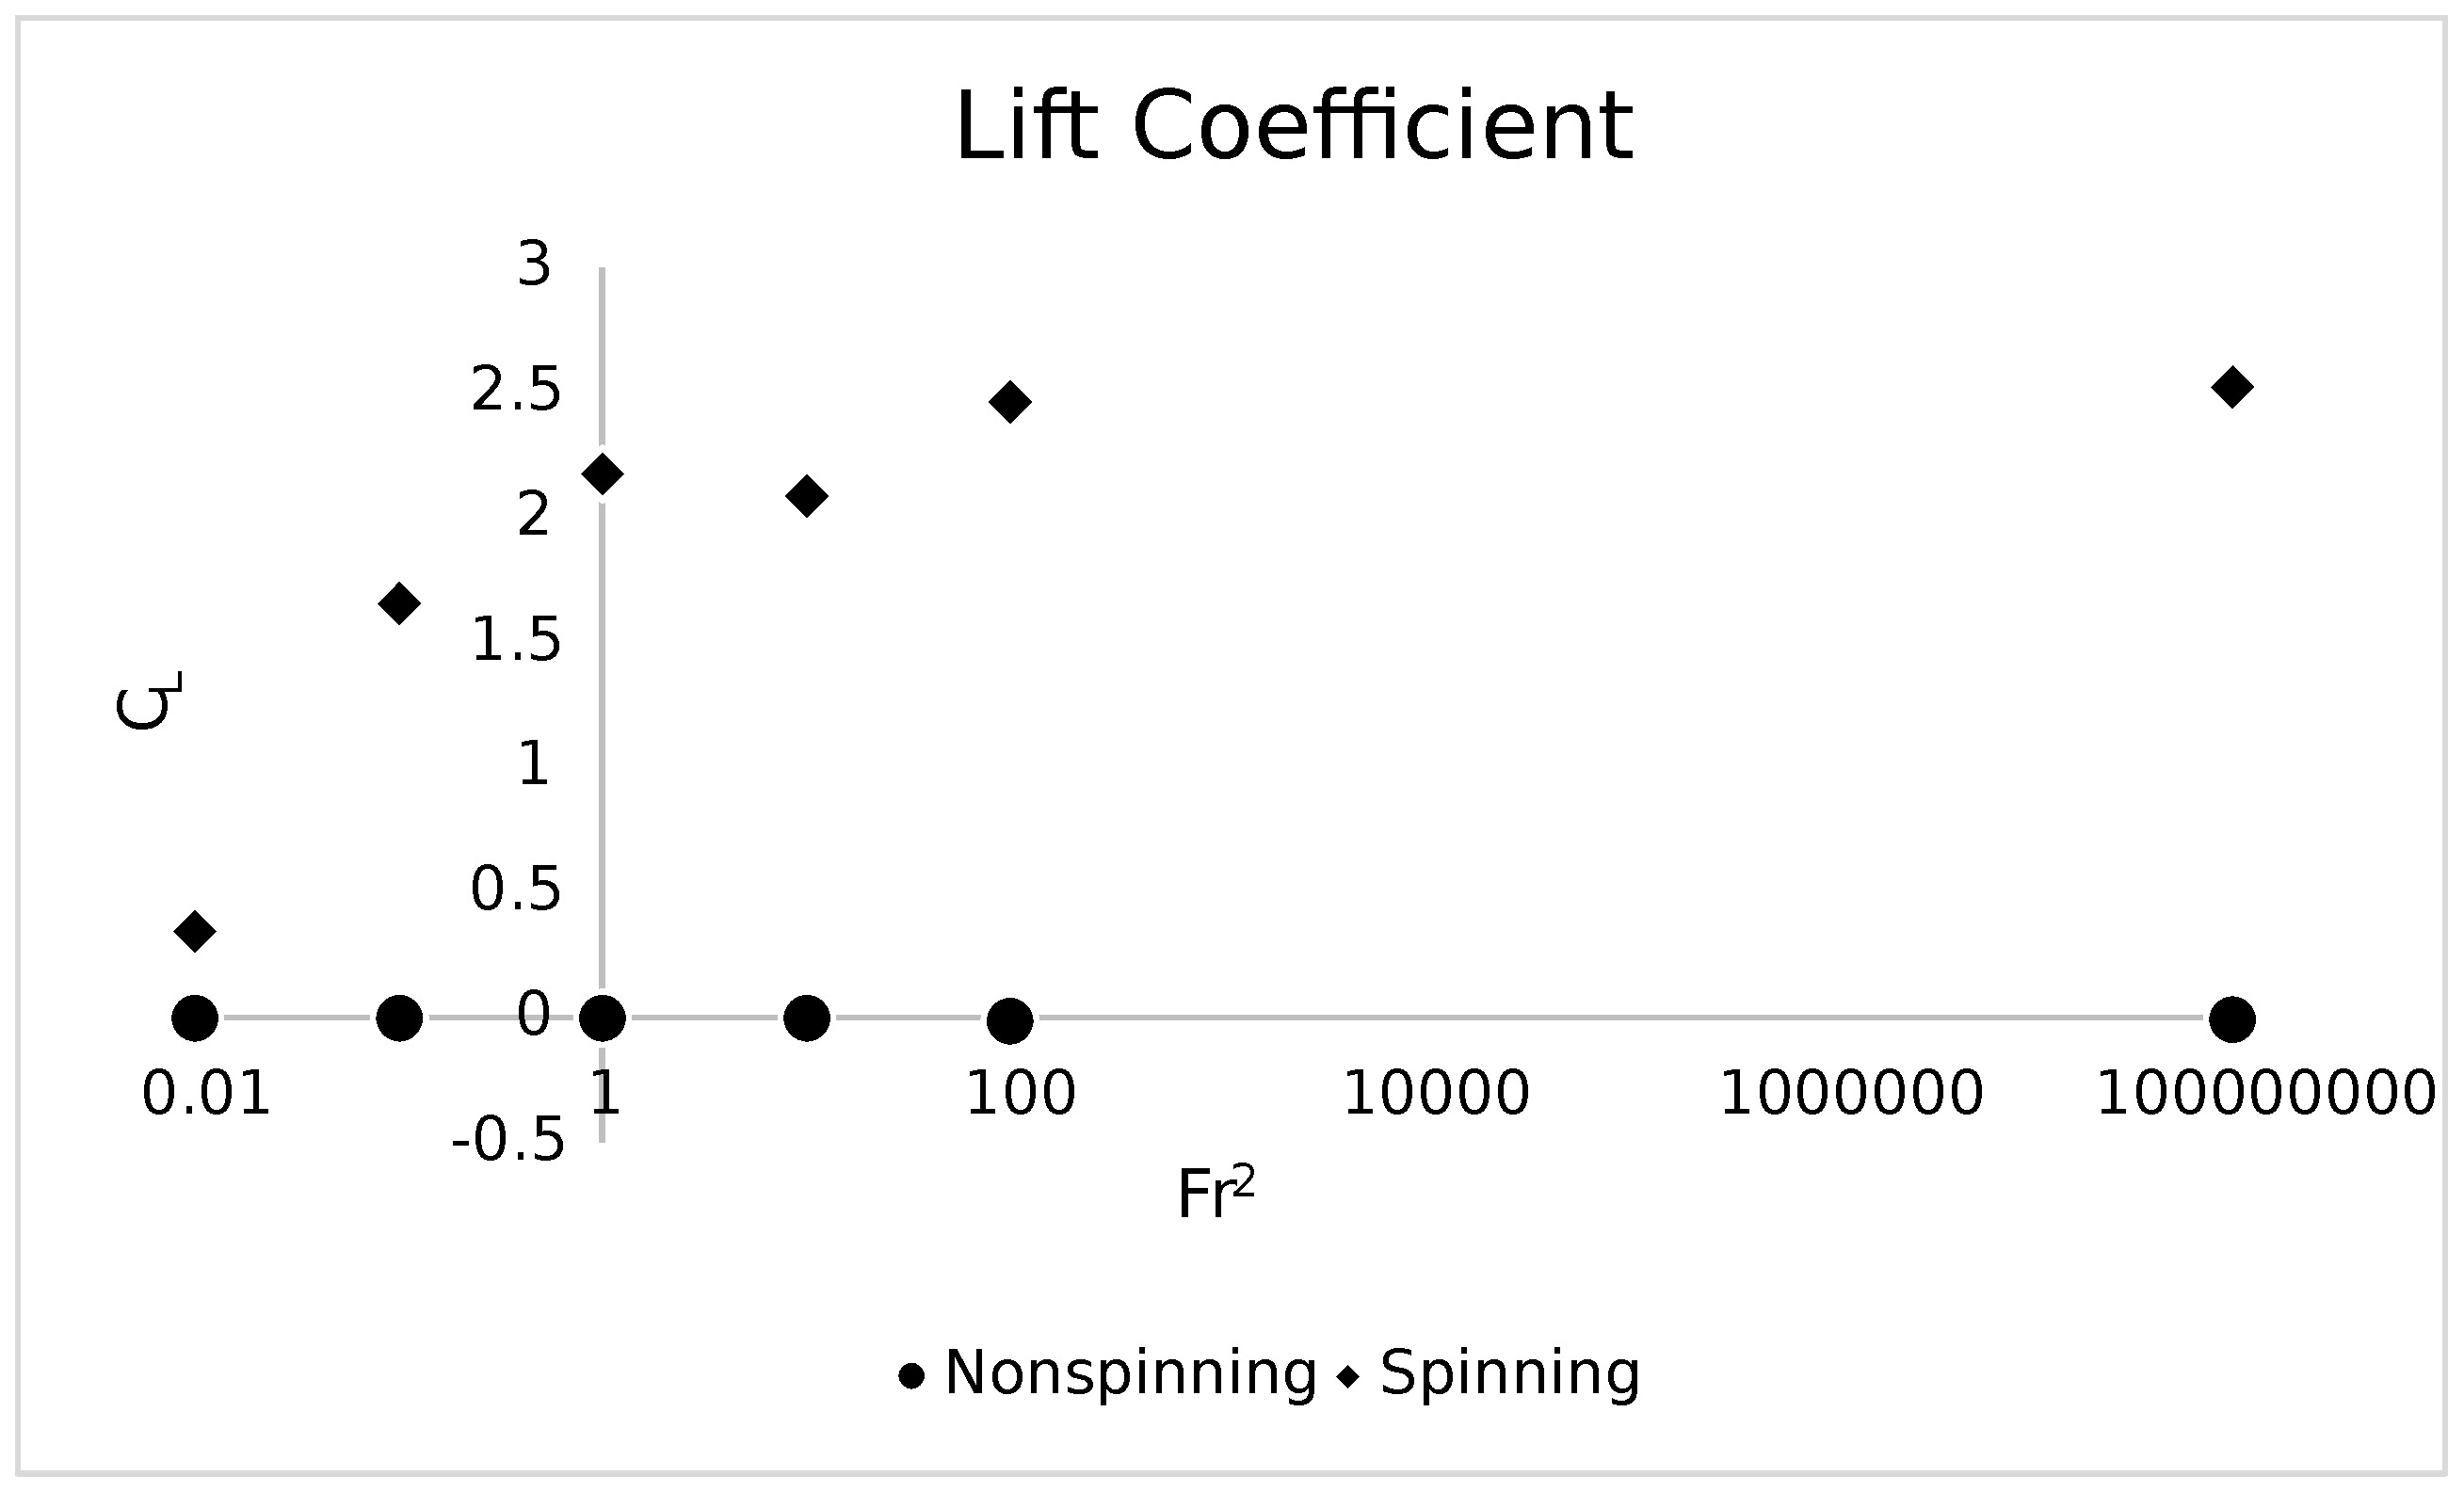
\includegraphics[width=\textwidth]{images/circle/ar1lift.eps}
        \caption{Lift coefficients}
        \label{fig:ar1lift}
    \end{subfigure}
    \caption{Mean drag and lift values for $\Omega^{\ast} = {0,1}$}
    \label{fig:circleforces}
\end{figure} 
\begin{figure}   
    \centering
        \begin{subfigure}[b]{0.25\textwidth}
        \centering
        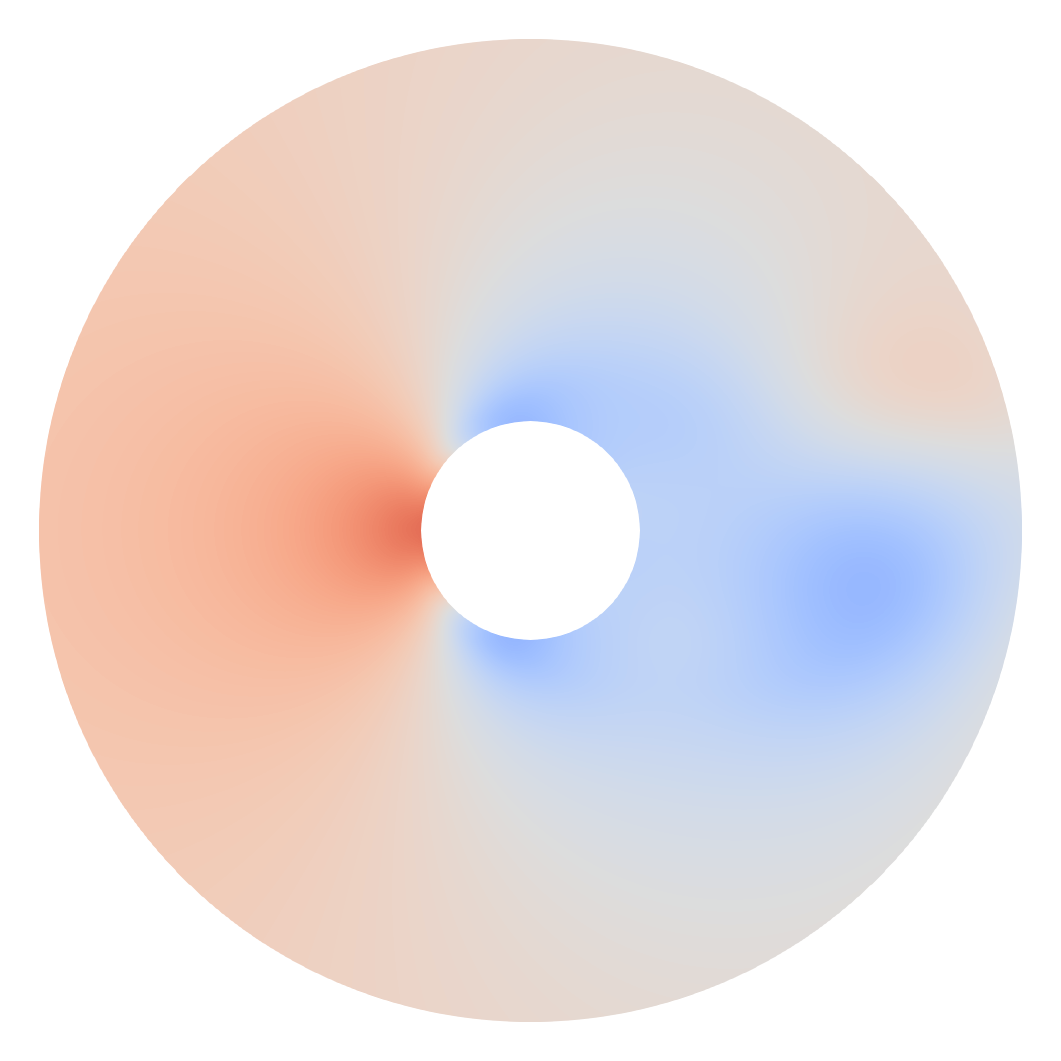
\includegraphics[width=\textwidth]{images/circle/ps0fsinf.png}
        \caption{$Fr^2 = \infty, \Omega^{\ast} = 0$}
        \label{fig:ps0fsinf}
    \end{subfigure}
    \hfill
    \begin{subfigure}[b]{0.25\textwidth}
        \centering
        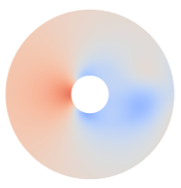
\includegraphics[width=\textwidth]{images/circle/ps0fs100.png}
        \caption{$Fr^2 = 100, \Omega^{\ast} = 0$}
        \label{fig:ps0fs100}
    \end{subfigure}
    \hfill
    \begin{subfigure}[b]{0.25\textwidth}
        \centering
        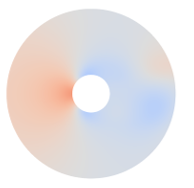
\includegraphics[width=\textwidth]{images/circle/ps0fs10.png}
        \caption{$Fr^2 = 10, \Omega^{\ast} = 0$}
        \label{fig:ps0fs10}
    \end{subfigure}
    
    \begin{subfigure}[b]{0.25\textwidth}
        \centering
        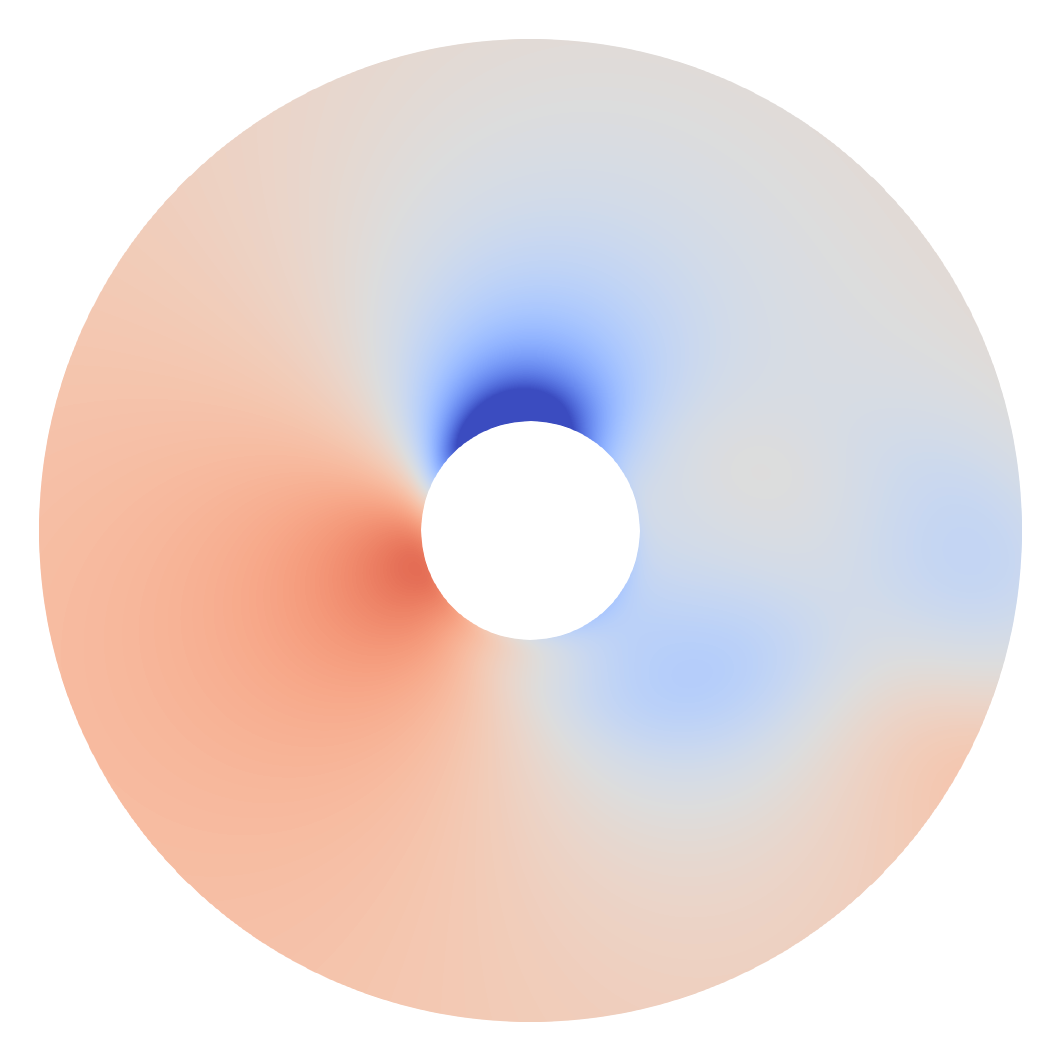
\includegraphics[width=\textwidth]{images/circle/ps1fsinf.png}
        \caption{$Fr^2 = \infty, \Omega^{\ast} = 1$}
        \label{fig:ps1fsinf}
    \end{subfigure}
    \hfill
    \begin{subfigure}[b]{0.25\textwidth}
        \centering
        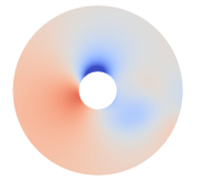
\includegraphics[width=\textwidth]{images/circle/ps1fs100.png}
        \caption{$Fr^2 = 100, \Omega^{\ast} = 1$}
        \label{ps1fs100}
    \end{subfigure}
    \hfill
    \begin{subfigure}[b]{0.25\textwidth}
        \centering
        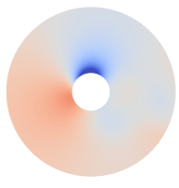
\includegraphics[width=\textwidth]{images/circle/ps1fs10.png}
        \caption{$Fr^2 = 10, \Omega^{\ast} = 1$}
        \label{fig:ps1fs10}
    \end{subfigure}

    \begin{subfigure}[b]{0.25\textwidth}
        \centering
        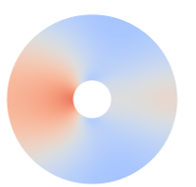
\includegraphics[width=\textwidth]{images/circle/ps0fs1.png}
        \caption{$Fr^2 = 1, \Omega^{\ast} = 0$}
        \label{fig:ps0fs1}
    \end{subfigure}
    \hfill
    \begin{subfigure}[b]{0.25\textwidth}
        \centering
        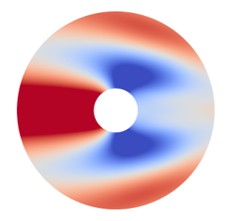
\includegraphics[width=\textwidth]{images/circle/ps0fs0p1.png}
        \caption{$Fr^2 = 0.1, \Omega^{\ast} = 0$}
        \label{fig:ps0fs0p1}
    \end{subfigure}
    \hfill
    \begin{subfigure}[b]{0.25\textwidth}
        \centering
        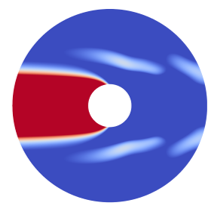
\includegraphics[width=\textwidth]{images/circle/ps0fs0p01.png}
        \caption{$Fr^2 = 0.01, \Omega^{\ast} = 0$}
        \label{fig:ps0fs0p01}
    \end{subfigure}

    \begin{subfigure}[b]{0.25\textwidth}
        \centering
        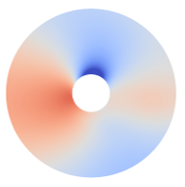
\includegraphics[width=\textwidth]{images/circle/ps1fs1.png}
        \caption{$Fr^2 = 1, \Omega^{\ast} = 1$}
        \label{fig:ps1fs1}
    \end{subfigure}
    \hfill
    \begin{subfigure}[b]{0.25\textwidth}
        \centering
        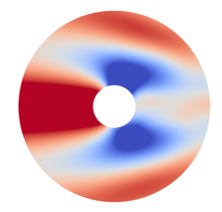
\includegraphics[width=\textwidth]{images/circle/ps1fs0p1.png}
        \caption{$Fr^2 = 0.1, \Omega^{\ast} = 1$}
        \label{fig:ps1fs0p1}
    \end{subfigure}
    \hfill
    \begin{subfigure}[b]{0.25\textwidth}
        \centering
        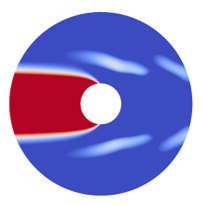
\includegraphics[width=\textwidth]{images/circle/ps1fs0p01.png}
        \caption{$Fr^2 = 0.01, \Omega^{\ast} = 1$}
        \label{fig:ps1fs0p01}
    \end{subfigure}
    
    \begin{subfigure}[b]{0.25\textwidth}
        \centering
        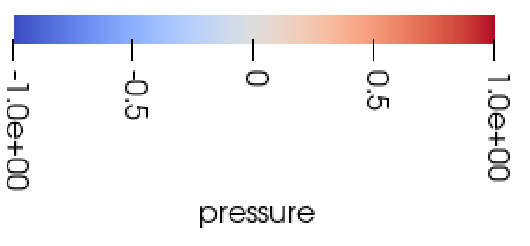
\includegraphics[width=\textwidth]{images/circle/p_scale.png}
        \caption*{}
    \end{subfigure}
    
    \caption{A comparison of the pressure fields for nonspinning and spinning circles}
    \label{fig:circle_pressure}
\end{figure}
\subsection{Flow structures}
We look at the y-velocity plot that Fig. \ref{fig:circle y-vel} shows. We observe that introducing spin does not significantly alter the flow at $Fr^2 < 1$. At $Fr^2 > 1$, the eddy wake is rotated clockwise, as expected. The plots show that the flow regime in both cases at $Fr^2 = 1$ is in transition. The vortex shedding that exists with lower stratification diminishes at $Fr^2 = 1$ as stratification increases. The plots show there is an optimal level of stratification for gravity propagation. The plots show that at the edges of our $Fr^2$ parameter space, the gravity waves do not propagate well. The gravity waves propagate best at around $Fr^2 = 1$. We observe periodic semi-circular patterns at $Fr^2 = 1, 0.1$ that are also observed in literatre \cite{ortiz-tarin_stratified_2019}.
 
We include schlerien plots (first derivative in density) in Fig. \ref{fig:circleschlerien}. Figure \ref{fig:circleschlerien2} shows some transitial $Fr^2$ results. The schlerien plots better capture the flow structures at higher $Fr^2$; the y-velocity plots do not fully capture the details of the vortex-shedding that occurs at high $Fr^2$. At $Fr^2 = 7, 10$, the schlerien plots show competition between a vortex-dominated-regime and an internal-gravity-wave regime. At these $Fr^2$ numbers, we see the formation of vortices and their breakdown, while in the internal-gravity-wave regime where $Fr^2 < 7$ there is no vortex-shedding. We see that the two phenomena are competing at $Fr^2 = 10$. Vortex-shedding is occurring, but is being suppressed. Gravity waves are present, but weak. This explains why in our time-series and ensemble-average plots the drag values do not settle to a steady value.
 
The reason the strength of the propagation of gravity waves as function of stratification is not linear is because there are two competing phenomena. The first phenomenon is the requirement of a restoring force for oscillation. This restoring forces comes from the density gradient, and the larger the density gradient, the larger the restoring force. The other phenomenon is the resistance of vertical motion due to stratification. This resistance increases with stratification. The combination of these competing phenomena result in an optimum level of stratification for gravity wave propagation. We observe that at low $Fr^2$, the IGW have little amplitude but do not dissipate easily. The reason for this is the high energy potential from high stratification is very sensitive to displacements. The IGW will still have small amplitudes, but the vertical high information-dependence across the domain will allow little dissipation. In the case of $Fr^2 = 0.01$, the dissipation is so weak that the IGW are spuriously reflecting off the boundaries.
 
The flow pattern we observe in the cases of $Fr^2 \in [7, 10]$ in which a wake whose scale is on the order of the cylinder breaks down into smaller-scale wakes. This feature is also observed in literature \cite{deng_drag_2022} for a nonspinning circle, who states this feature does not exist in homogeneous flows. This feature does not exist in unstratified flows because there is no potential energy barrier resisting vertical motion like there is in stratified flow. In stratified flows, the resistance to vertical motion causes the wakes and vorticies to break down into features with less vertical displacement. An observation that confirms the earlier mathematically extracted hypothesis from equation \ref{eq:nondim NBV} that as we increase our stratification, our Brunt–Väisälä frequency increases. This phenomenon manifests itself in the decrease in the wavelength of the gravity waves in the plots.

\begin{figure}   
    \centering
        \begin{subfigure}[b]{0.32\textwidth}
        \centering
        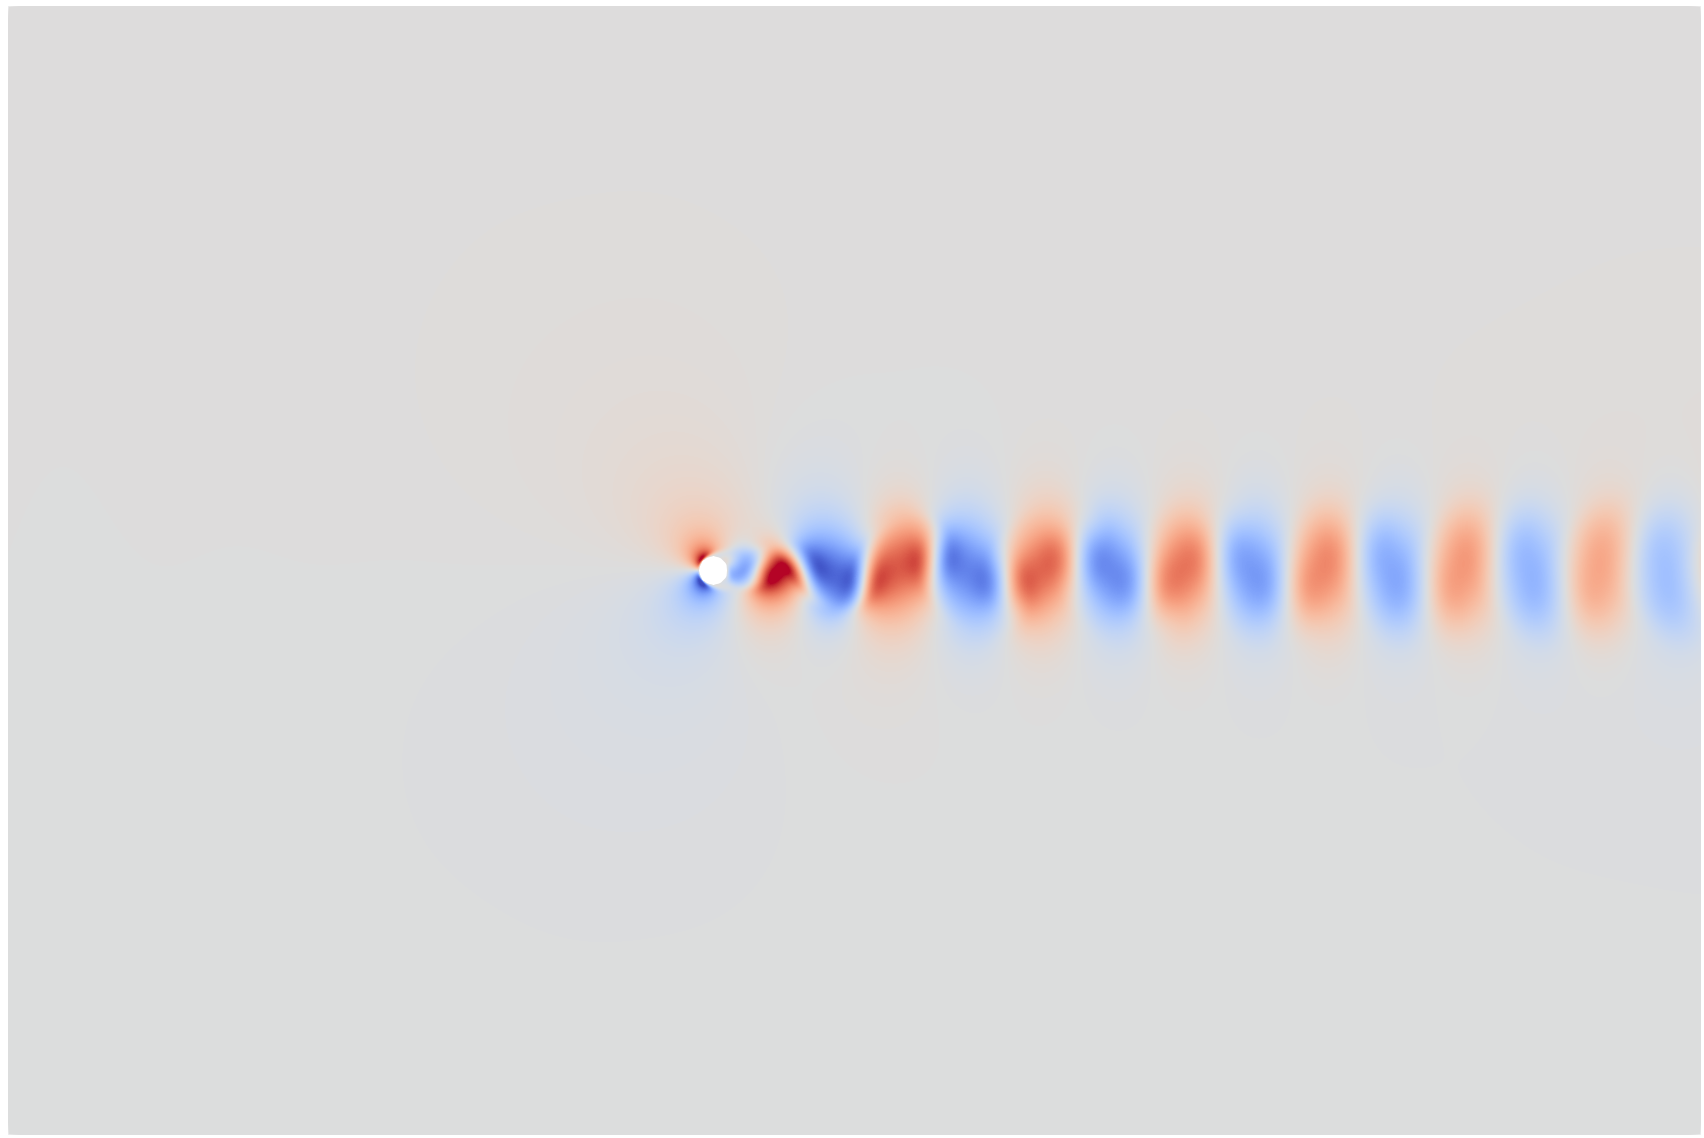
\includegraphics[width=\textwidth]{images/circle/av0fsinf.png}
        \caption{$Fr^2 = \infty, \Omega^{\ast} = 0$}
        \label{fig:av0fsinf}
    \end{subfigure}
    \hfill
    \begin{subfigure}[b]{0.32\textwidth}
        \centering
        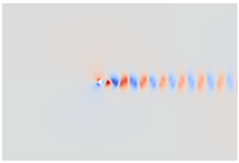
\includegraphics[width=\textwidth]{images/circle/av0fr10.png}
        \caption{$Fr^2 = 100, \Omega^{\ast} = 0$}
        \label{fig:av0frs100}
    \end{subfigure}
    \hfill
    \begin{subfigure}[b]{0.32\textwidth}
        \centering
        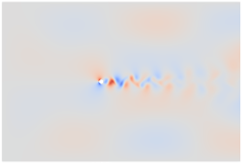
\includegraphics[width=\textwidth]{images/circle/av0fr3.png}
        \caption{$Fr^2 = 10, \Omega^{\ast} = 0$}
        \label{fig:av0frs10}
    \end{subfigure}
    
    \begin{subfigure}[b]{0.32\textwidth}
        \centering
        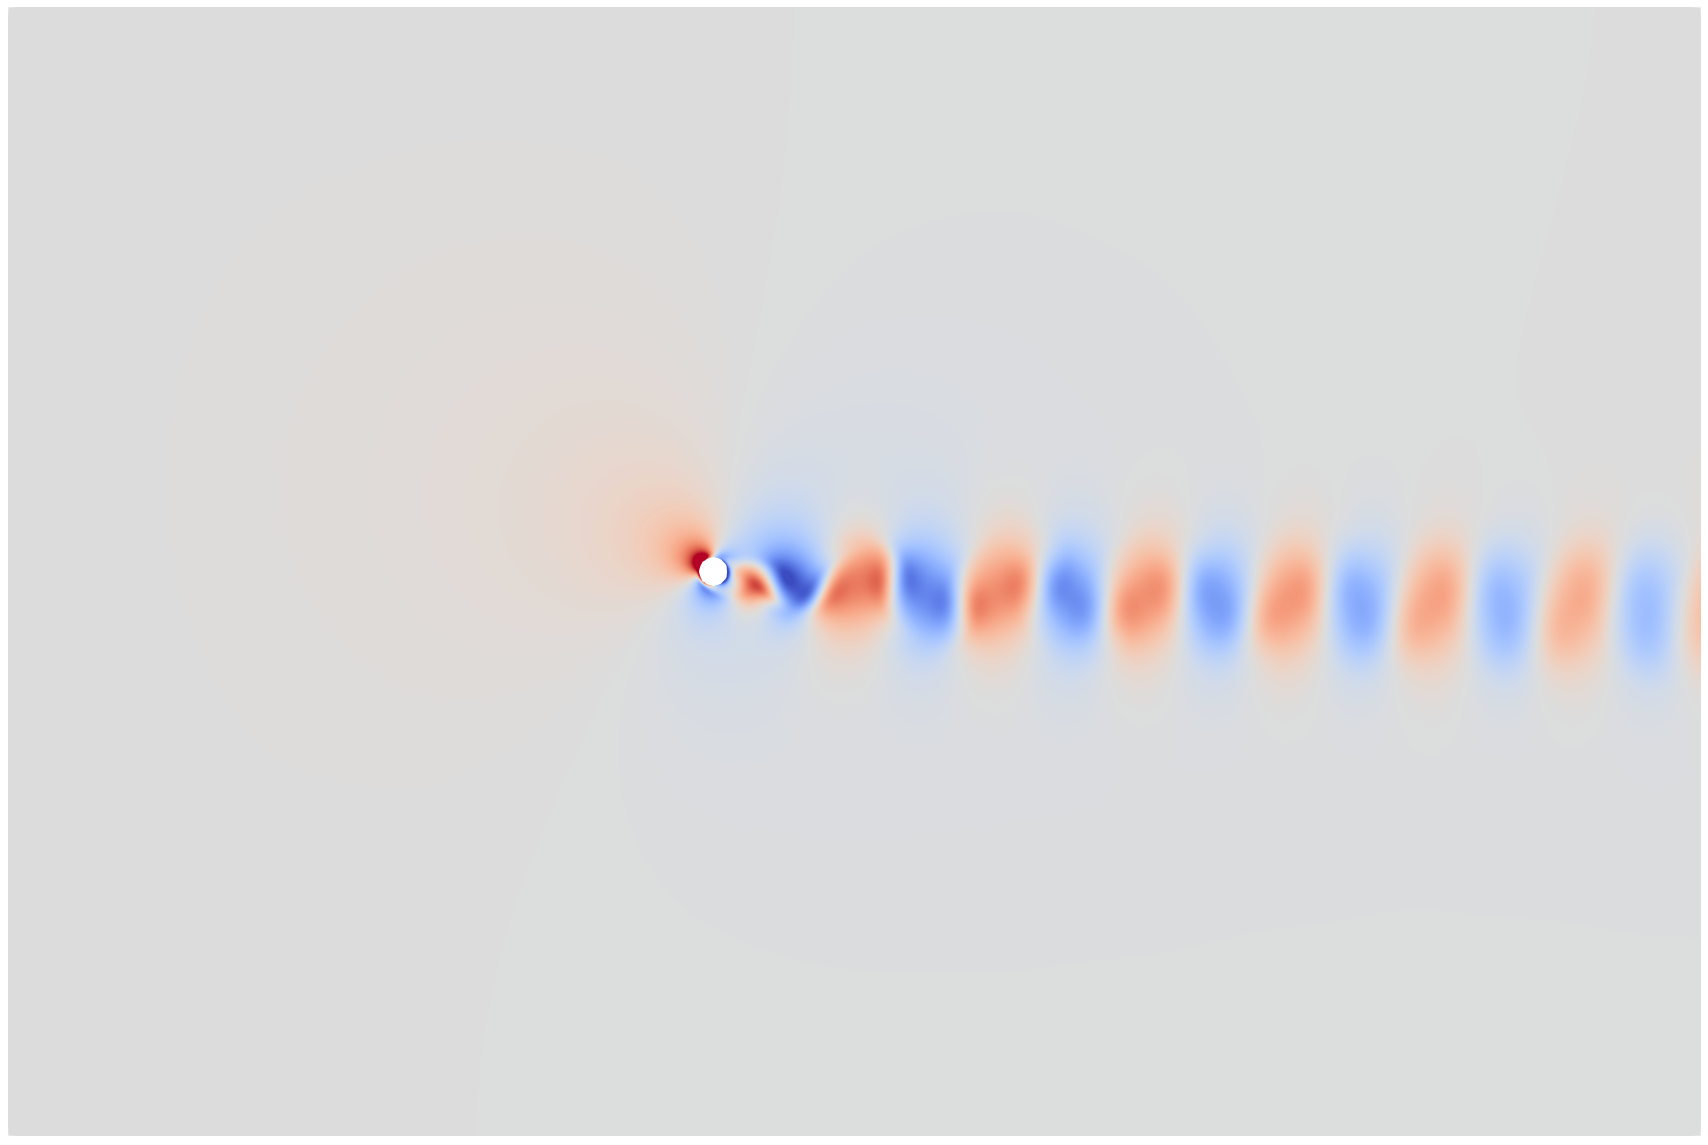
\includegraphics[width=\textwidth]{images/circle/av1fsinf.png}
        \caption{$Fr^2 = \infty, \Omega^{\ast} = 1$}
        \label{fig:av1fsinf}
    \end{subfigure}
    \hfill
    \begin{subfigure}[b]{0.32\textwidth}
        \centering
        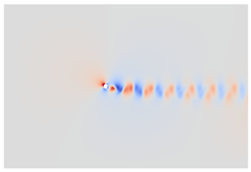
\includegraphics[width=\textwidth]{images/circle/av1fr10.png}
        \caption{$Fr^2 = 100, \Omega^{\ast} = 1$}
        \label{av1frs100}
    \end{subfigure}
    \hfill
    \begin{subfigure}[b]{0.32\textwidth}
        \centering
        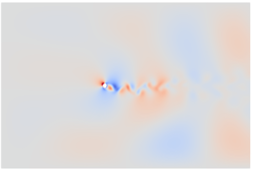
\includegraphics[width=\textwidth]{images/circle/av1fr3.png}
        \caption{$Fr^2 = 10, \Omega^{\ast} = 1$}
        \label{fig:av1frs10}
    \end{subfigure}

    \begin{subfigure}[b]{0.32\textwidth}
        \centering
        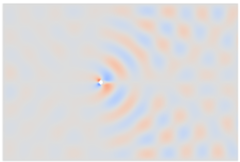
\includegraphics[width=\textwidth]{images/circle/av0fr1.png}
        \caption{$Fr^2 = 1, \Omega^{\ast} = 0$}
        \label{fig:av0frs1}
    \end{subfigure}
    \hfill
    \begin{subfigure}[b]{0.32\textwidth}
        \centering
        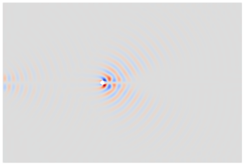
\includegraphics[width=\textwidth]{images/circle/av0fr0p3.png}
        \caption{$Fr^2 = 0.1, \Omega^{\ast} = 0$}
        \label{fig:av0frs0p1}
    \end{subfigure}
    \hfill
    \begin{subfigure}[b]{0.32\textwidth}
        \centering
        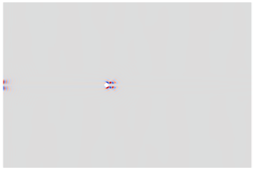
\includegraphics[width=\textwidth]{images/circle/av0fr0p1.png}
        \caption{$Fr^2 = 0.01, \Omega^{\ast} = 0$}
        \label{fig:av0frs0p01}
    \end{subfigure}

    \begin{subfigure}[b]{0.32\textwidth}
        \centering
        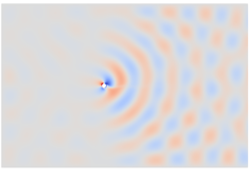
\includegraphics[width=\textwidth]{images/circle/av1fr1.png}
        \caption{$Fr^2 = 1, \Omega^{\ast} = 1$}
        \label{fig:av1frs1}
    \end{subfigure}
    \hfill
    \begin{subfigure}[b]{0.32\textwidth}
        \centering
        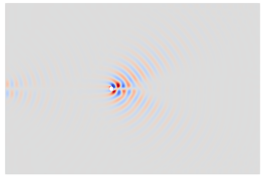
\includegraphics[width=\textwidth]{images/circle/av1fr0p3.png}
        \caption{$Fr^2 = 0.1, \Omega^{\ast} = 1$}
        \label{fig:av1frs0p1}
    \end{subfigure}
    \hfill
    \begin{subfigure}[b]{0.32\textwidth}
        \centering
        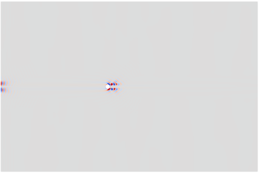
\includegraphics[width=\textwidth]{images/circle/av1fr0p1.png}
        \caption{$Fr^2 = 0.01, \Omega^{\ast} = 1$}
        \label{fig:av1frs0p01}
    \end{subfigure}
    
    \begin{subfigure}[b]{0.32\textwidth}
        \centering
        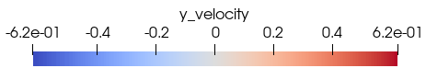
\includegraphics[width=\textwidth]{images/circle/scale.png}
        \caption*{}
    \end{subfigure}
    
    \caption{A comparison of the y-velocity fields for nonspinning and spinning circles}
    \label{fig:circle y-vel}
\end{figure}

\begin{figure}
    \centering
    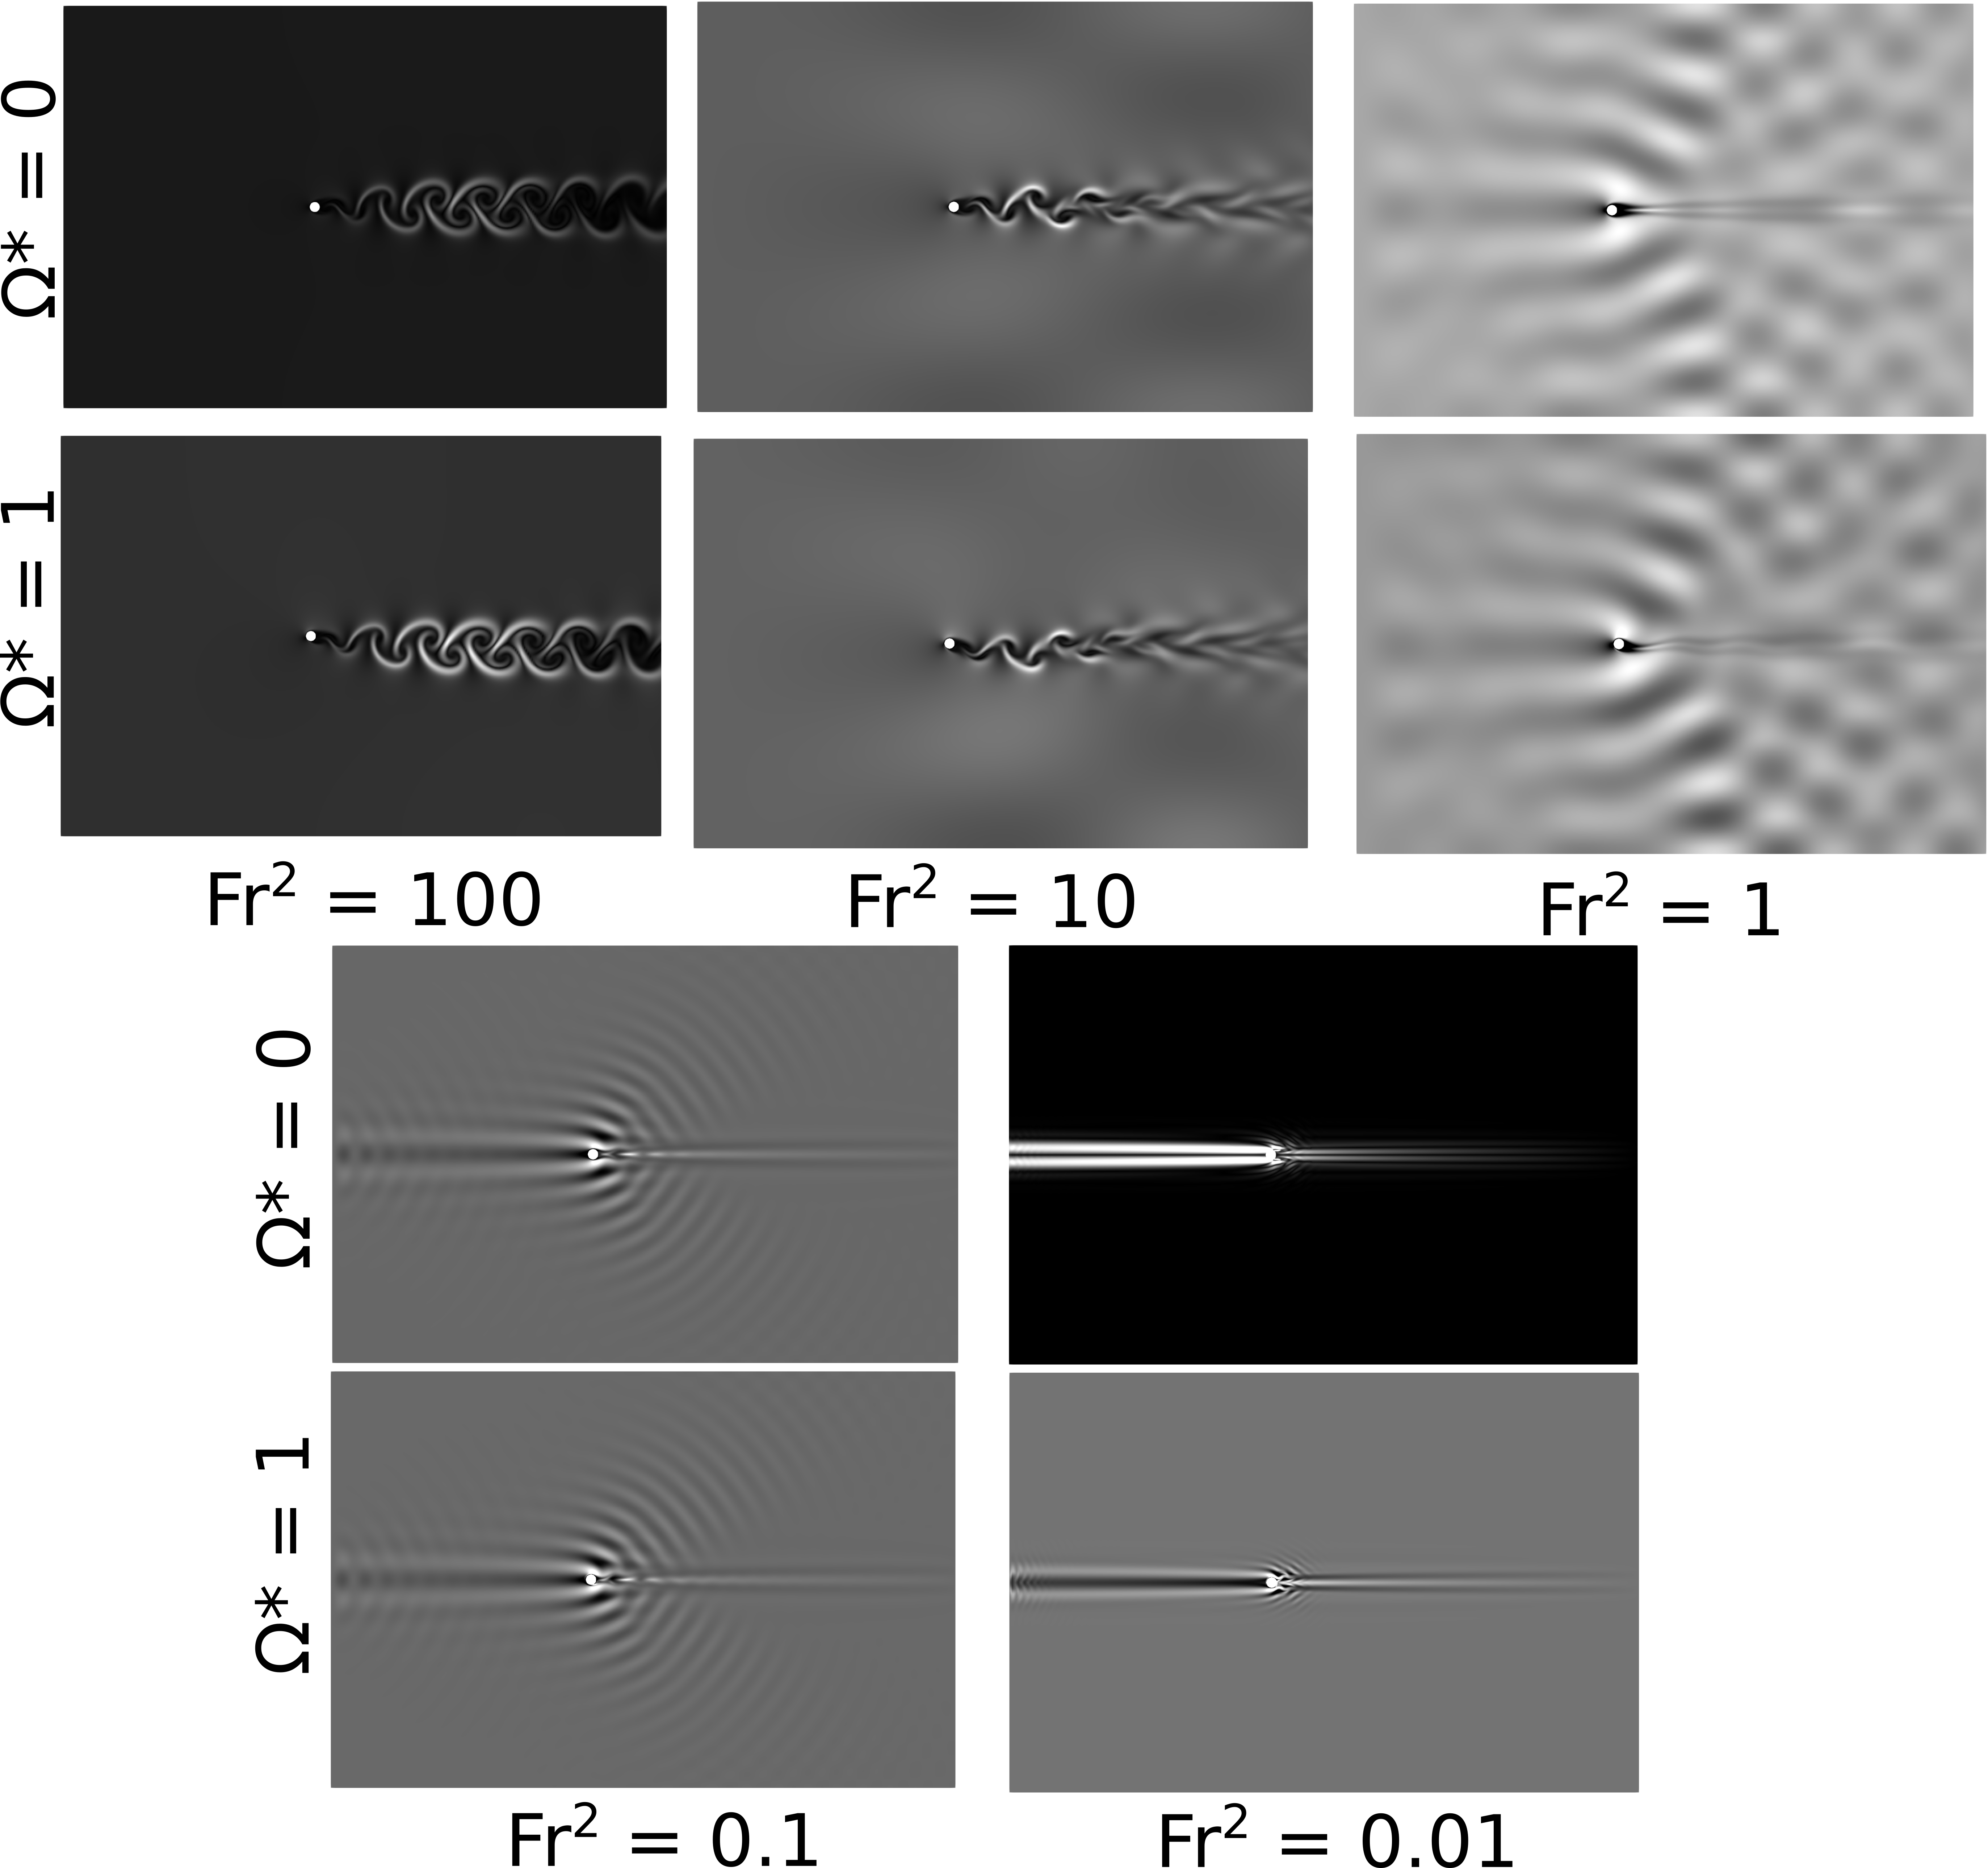
\includegraphics[width = \textwidth]{images/circle/circleschlerien.png}
    \caption{A comparison of the Schlerien fields for nonspinning and spinning circles}
    \label{fig:circleschlerien}
\end{figure}

\begin{figure}
    \centering
    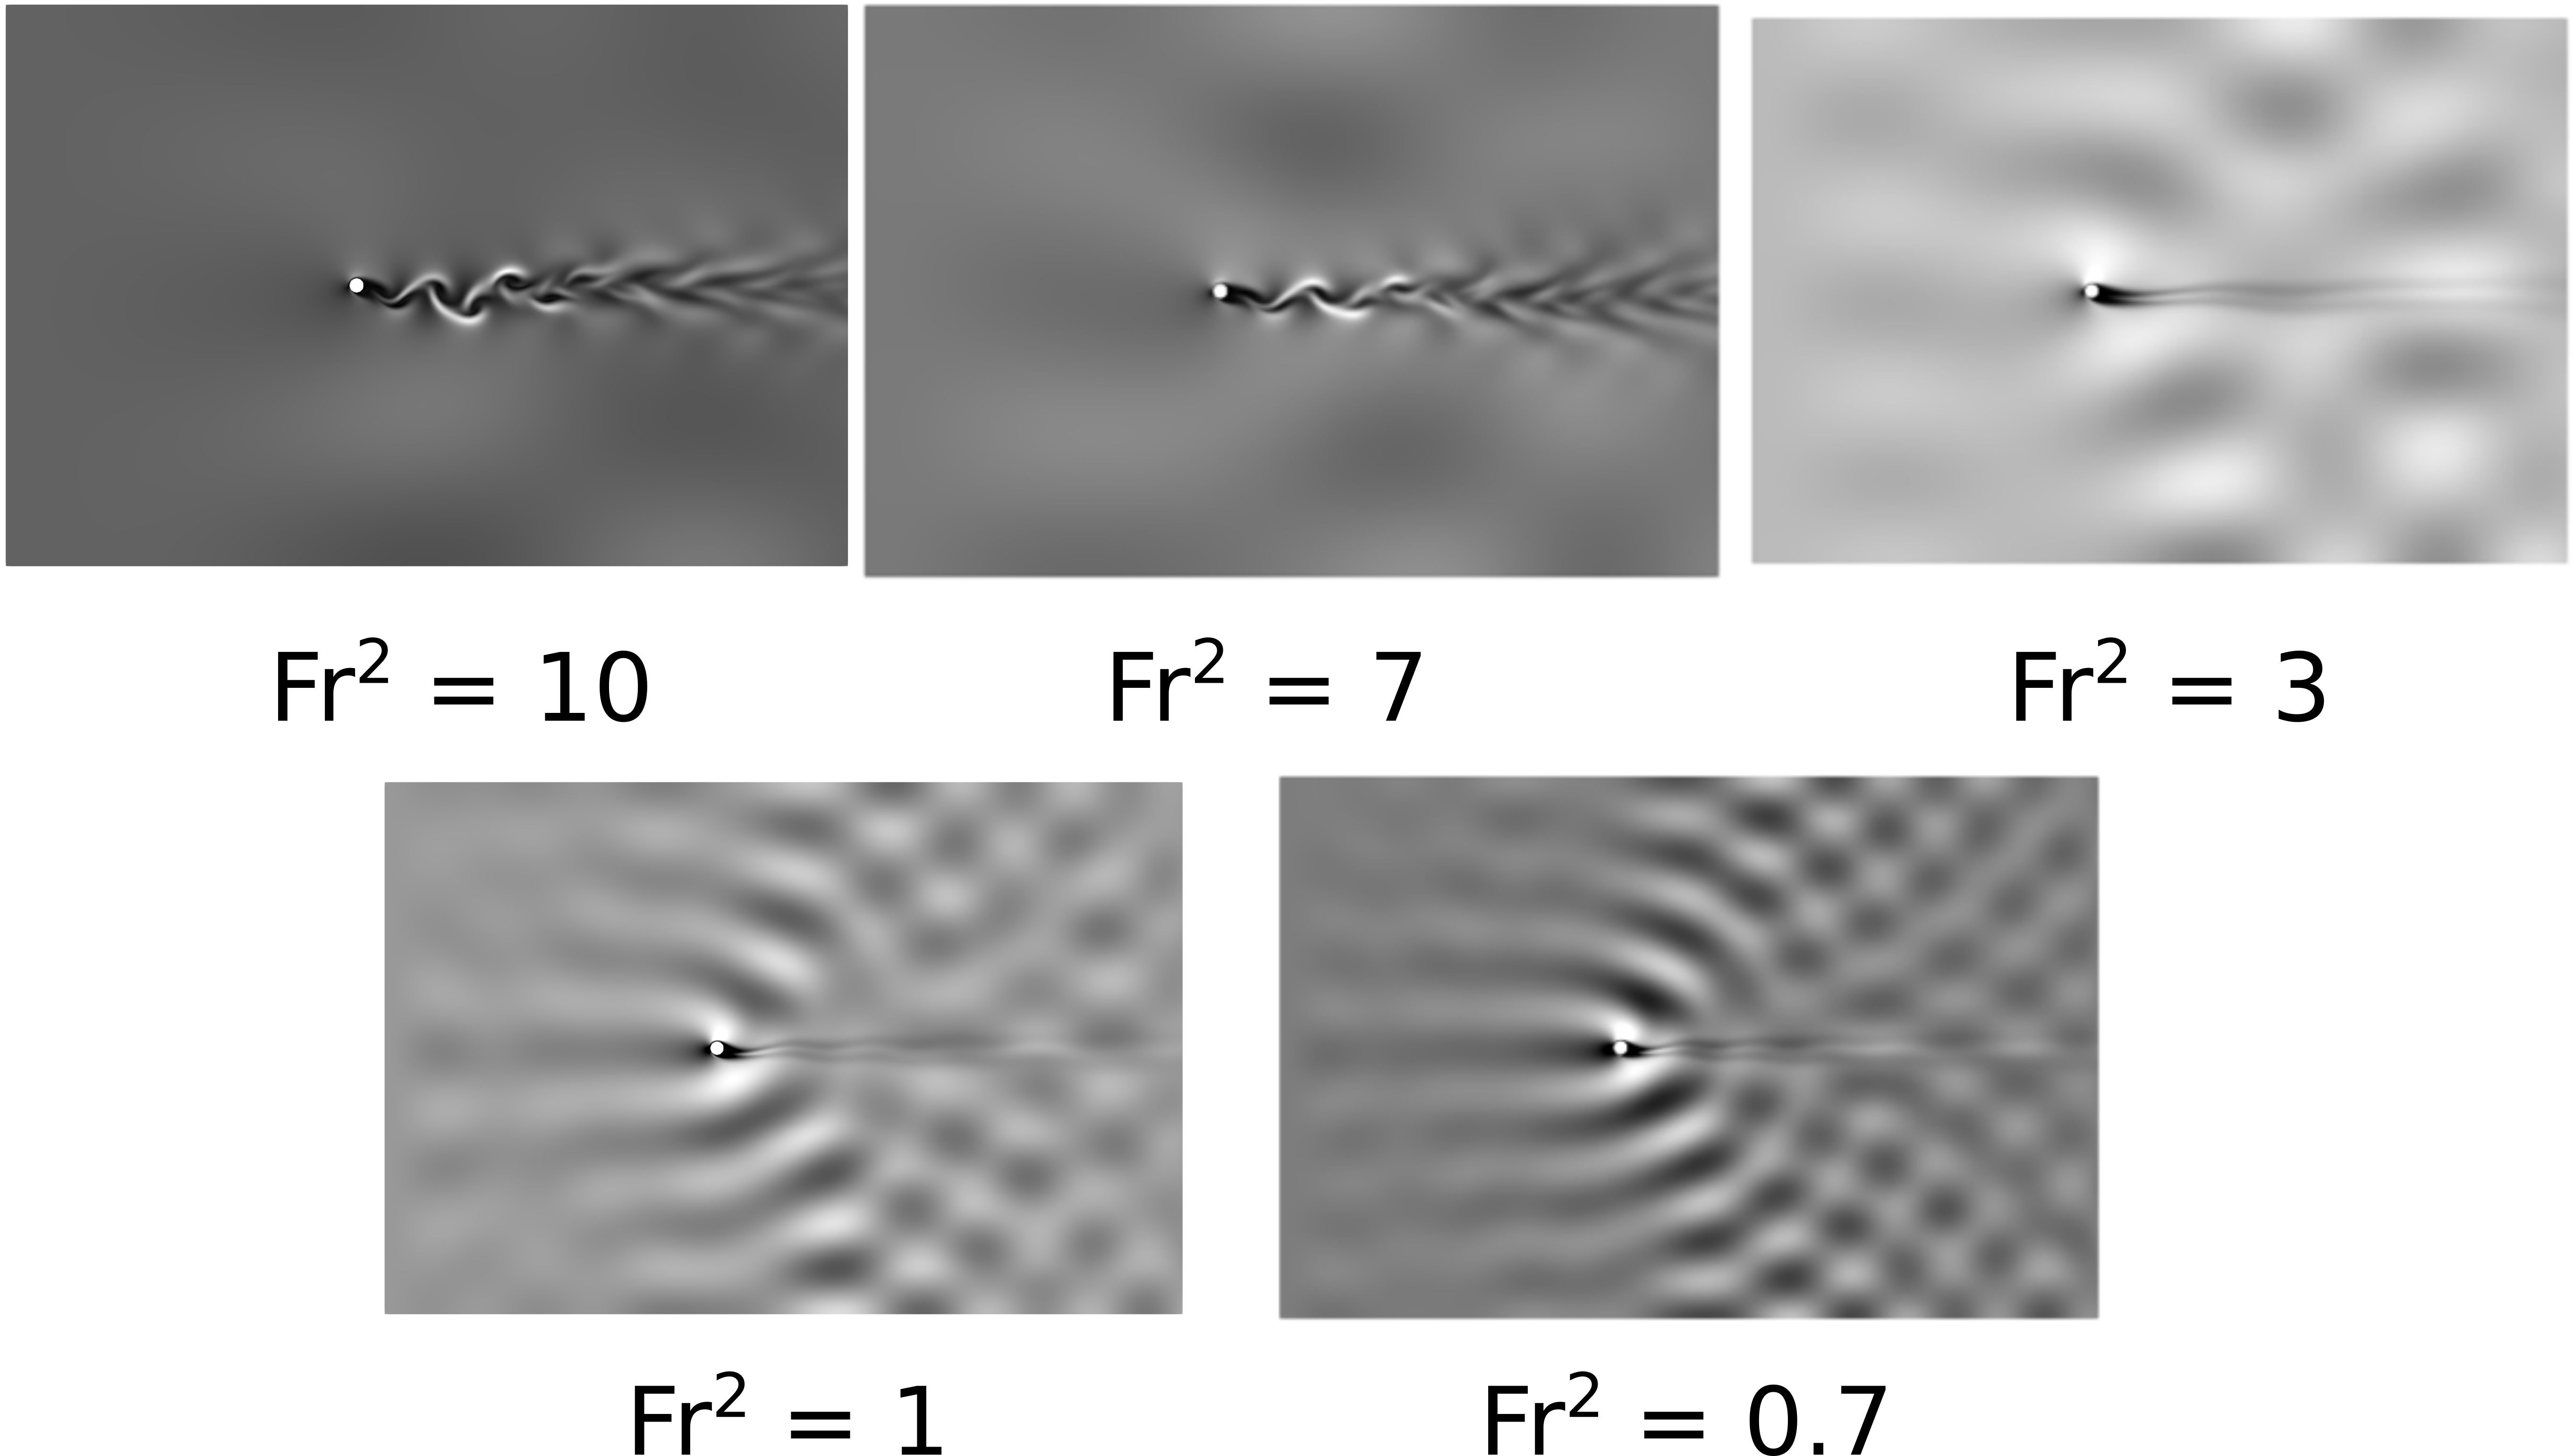
\includegraphics[width = \textwidth]{images/circle/circleschlerien2.png}
    \caption{A close look of the Schlerien plots at the transition with spin}
    \label{fig:circleschlerien2}
\end{figure}

